\documentclass[fontset=windows,openany,UTF8]{ctexbook}

\usepackage{caption}
\DeclareCaptionFont{sfive}{\zihao{-5}}
\captionsetup[figure]{format=hang,font={sfive},labelsep=quad}
\captionsetup[table]{format=hang,font={sfive,bf},labelsep=quad,skip=5pt}

\setlength\marginparwidth{0.8in}
\addtolength\marginparsep{3mm}
\usepackage{xcolor}
\usepackage{zhlipsum}

\usepackage{graphicx}

\usepackage[papersize={185 true mm, 260 true mm},top=10mm,bottom=5mm,inner=25 true mm,outer=5mm,includeall]{geometry}
\usepackage{listings}
\usepackage{url}
\lstset{
    basicstyle=\ttfamily\scriptsize,
    numbers=left, 
    numberstyle= \tiny, 
    keywordstyle= \color{ blue!70},
    commentstyle= \color{red!50!green!50!blue!50}, 
    frame=shadowbox, % 阴影效果
    rulesepcolor= \color{ red!20!green!20!blue!20} ,
    escapeinside=``, % 英文分号中可写入中文
    xleftmargin=2em,xrightmargin=2em, aboveskip=1em,
    framexleftmargin=2em,
    breaklines      =   true, 
} 

\ctexset{section={name={,}, format={\zihao{-3}},beforeskip={15pt plus 1pt minus 1pt}, afterskip={12pt
plus 1pt minus 1pt},aftername={\quad}}}

\ctexset{subsection={name={,},format={\indent\zihao{-4}\sffamily}}}
\ctexset{chapter={name={第,章~},pagestyle=empty, format={\centering},nameformat={\zihao{3}\bfseries},titleformat={\zihao{3}\bfseries}, number=\arabic{chapter},
beforeskip={12pt},afterskip={32pt}, aftername={\quad}}}
%%%
\ctexset{appendix={name={附录~}}}%,number=\arabic{chapter}}}

\ctexset{indexname={索\qquad 引},tablename={表},figurename={图},contentsname={目\qquad 录}}

\begin{document}
\title{人工智能教材}
\author{作者}
\date{\vspace*{3in}出版社名称}

\maketitle
\thispagestyle{empty}
\frontmatter

%\begin{center}
%\textbf{\bfseries\zihao{3}内容提要}
%\end{center}
%\
\chapter*{内容提要}

内容提要说明本书的主要内容、编写特色以及适用对象。
\clearpage

\chapter*{前\qquad 言}
前言即作者想对读者说的话,教材的前言一般包括写作背景、写作思路、本书的组织架构、本书配套的辅助资料和致谢等内容。


{\centering\tableofcontents}

\mainmatter

\chapter{基于计算机的问题求解}
\noindent【内容导读】 因特网梅森素数大搜索
\addcontentsline{toc}{section}{内容导读}

\section{问题描述与抽象}
\subsection{问题描述}
如果在正文中对应的重难点内容,制作了微视频,我们可以制作二维码放书的边栏,见右侧\marginpar{\color{cyan}\textbf{微视频}\\ 求余运算的应用举例}如果在正文中对应的重难点内容,制作了微视频,我们可以制作二维码放书的边栏,见右侧如果在正文中对应的重难点内容,制作了微视频,我们可以制作二维码放书的边栏,见右侧如果在正文中对应的重难点内容,制作了微视频,我们可以制作二维码放书的边栏,见右侧如果在正文中对应的重难点内容,制作了微视频,我们可以制作二维码放书的边栏,见右侧如果在正文中对应的重难点内容,制作了微视频,我们可以制作二维码放书的边栏,见右侧如果在正文中对应的重难点内容,制作了微视频,我们可以制作二维码放书的边栏,见右侧如果在正文中对应的重难点内容,制作了微视频,我们可以制作二维码放书的边栏,见右侧如果在正文中对应的重难点内容,制作了微视频,我们可以制作二维码放书的边栏,见右侧如果在正文中对应的重难点内容,制作了微视频,我们可以制作二维码放书的边栏,见右侧如果在正文中对应的重难点内容,制作了微视频,我们可以制作二维码放书的边栏,见右侧如果在正文中对应的重难点内容,制作了微视频,我们可以制作二维码放书的边栏,见右侧如果在正文中对应的重难点内容,制作了微视频,我们可以制作二维码放书的边栏,见右侧如果在正文中对应的重难点内容,制作了微视频,我们可以制作二维码放书的边栏,见右侧如果在正文中对应的重难点内容,制作了微视频,我们可以制作二维码放书的边栏,见右侧如果在正文中对应的重难点内容,制作了微视频,我们可以制作二维码放书的边栏,见右侧如果在正文中对应的重难点内容,制作了微视频,我们可以制作二维码放书的边栏,见右侧如果在正文中对应的重难点内容,制作了微视频,我们可以制作二维码放书的边栏,见右侧如果在正文中对应的重难点内容,制作了微视频,我们可以制作二维码放书的边栏,见右侧
\begin{figure}[h]
\centering\Huge \fbox{swdt.eps}
\caption{图题小五号宋体}
\end{figure}
\begin{table}[h]
\caption{表题小五号黑体}
\centering\Huge \fbox{此处为表格}
\end{table}

\section{标题}

\section{标题}

\section{本章知识点}
% \includegraphics{swdt.png}

\section{推荐读物}

\section*{实验\thechapter}
\addcontentsline{toc}{section}{实验\thechapter}

\section*{习题\thechapter}
\addcontentsline{toc}{section}{习题\thechapter}


\chapter{标题}

\section{自定义镜像训练}

\subsection{自定义镜像概述}

ModelArts 提供了多种预置引擎,但是当用户对深度学习引擎、开发库有特殊需求的场景的时候,预置引擎已经不能满足用户需求。此时用户可以使用 ModelArts 自定义镜像这个功能来达到自定义运行引擎的目的。

ModelArts 底层采用容器技术,自定义镜像指的是用户自行制作容器镜像并在 ModelArts 上运行。自定义镜像功能支持自由文本形式的命令行参数和环境变量,因此灵活性比较高,便于支持任意计算引擎的作业启动需求。

文中出现的英文缩略词意思分别为:SWR--华为云容器镜像服务,OBS--华为云对象存储服务

\subsection{介绍}

\subsubsection{docker}

Docker是一个开源的引擎,可以轻松的为任何应用创建一个轻量级的、可移植的、自给自足的容器。容器镜像服务兼容原生Docker,支持使用Docker CLI和原生API管理容器镜像。了解更多的docker知识参考文档\url{https://docs.docker.com/}

\subsubsection{swr}

容器镜像服务(Software Repository for Container,简称SWR)是一种支持镜像全生命周期管理的服务,提供简单易用、安全可靠的镜像管理功能,包括镜像的上传、下载、删除等。

SWR提供私有镜像库,并支持细粒度的权限管理,可以为不同用户分配相应的访问权限(读取、编辑、管理)。SWR还支持容器镜像版本更新自动触发部署。您只需要为镜像设置一个触发器,通过触发器,可以在每次镜像版本更新时,自动更新云容器引擎(CCE)中使用该镜像部署的应用。

您可以通过控制台、API使用容器镜像服务。

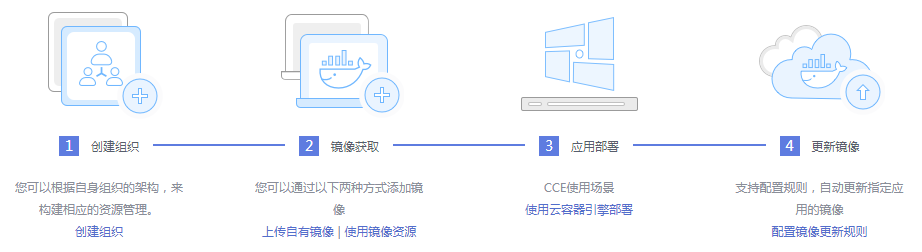
\includegraphics[scale=0.5]{./assets/swr1.png}  

\subsection{使用容器镜像服务}

\subsubsection{自定义镜像功能使用步骤}

ModelArts中使用自定义功能步骤如下:

1. 制作自定义镜像。

2. 传自定义镜像到华为云 SWR。

3. 在 ModelArts 上使

\subsubsection{制作自定义镜像}

制作自定义镜像时,需要往镜像中添加一些必要的深度学习库及用户编写的脚本等。

\subsubsection{自定义镜像规范要求}

1. 自定义镜像必须基于ModelArts官方提供的基础镜像,支持的基础镜像请参考基础镜像包。

2. 自定义镜像中不能包含恶意代码。

3. 基础镜像中的部分内容不能改变,包括“/bin”、“/sbin”、“/usr”、“/lib(64)”下的所有文件,“/etc”下的部分重要配置文件,以及“\$HOME”下的ModelArts小工具。

4. 不可以新增属主为`“root”`且权限包含“setuid”或“setgid”位的文件。
自定义镜像大小不能超过9.5GB。

5. 日志文件输出,为保证日志内容可以正常显示,日志信息需要打印到标准输出。

\subsection{基础镜像包}

基础镜像中有一些必要的工具,用户需要基于ModelArts官方提供的基础镜像来制作自定义镜像。
ModelArts将持续更新基础镜像版本,基础镜像更新后,对于兼容性更新,用户还可以继续使用旧的镜像;对于不兼容性更新,基于旧版本制作的自定义镜像将不能在ModelArts上运行,但已经审核过的自定义镜像可以继续使用。
当用户发现自定义镜像审核不通过,并且审核日志中出现基础镜像不匹配的错误信息时,需要使用新的基础镜像重新制作镜像。

基础镜像基础组件:

run\_train.sh : 训练启动引导脚本。实现了代码目录下载,执行训练命令、重定向训练日志输出、以及训练命令结束后上传日志文件至OBS的功能。

utils.sh : 工具脚本。“run\_train.sh”脚本依赖此脚本。提供了SK解密,代码目录下载,日志文件上传等方法。

ip\_mapper.py:网卡地址获取脚本。默认获取ib0网卡地址IP,训练代码可以使用ib0网卡的IP加速网络通信。

dls-downloader.py:OBS下载脚本。“utils.sh”脚本依赖此脚本。

完整的基础镜像内容可参考:\url{https://github.com/huaweicloud/ModelArts-Lab/tree/master/docs/custom_image/custom_base}

举一例子:


\lstset{language=bash}
    \begin{lstlisting}
FROM dls.io/dls/ubuntu_base:16.04-latest

ARG download
ARG username
ARG usergroup
ARG workname
ARG workgroup

RUN groupadd -g 1100 Misplaced &username -m -u 1100 -g 1100 -s /bin/bash $username &&\
  groupadd -g 1101 Misplaced &workname -m -u 1101 -g 1101 -s /bin/bash $workname && \
  mkdir /cache && chown -R workname:workgroup /cache && chmod 755 /cache

RUN mv /etc/apt/sources.list /etc/apt/sources.list~ && \
  wget ${download}/dls-release/ubuntu-16.04/ci-config/sources.list -P /etc/apt/ && \
  apt-get update && \
  apt-get install -y python-pip \
    libcurl4-openssl-dev && \
  echo "" > /etc/apt/apt.conf && \
  rm -f /etc/apt/sources.list && \
  rm -rf /var/lib/apt/lists/* && \
  mv /etc/apt/sources.list~ /etc/apt/sources.list && \
  chmod -R -s /usr/local/lib

RUN mkdir -p /home/install && cd /home/install && \
  wget $download/dls-release/ubuntu-16.04/dls-tools-master/latest/dls-decryptor && \
  chown root:root dls-decryptor && \
  chmod 4755 dls-decryptor && \
  mv dls-decryptor /usr/bin/ && \
  wget $download/dls-release/ubuntu-16.04/dls-tools-master/latest/dls-dns-fixer.tar.gz && \
  tar -xvzf dls-dns-fixer.tar.gz && chown root:root dls-dns-fixer && \
  chmod 6755 dls-dns-fixer && mv -v dls-dns-fixer /usr/bin/ && \
  wget $download/dls-release/ubuntu-16.04/dls-tools-master/latest/dls-pipe.tar.gz && \
  tar -xzf dls-pipe.tar.gz && chown 1100:1100 modelarts-pipe &&  chmod 6755 modelarts-pipe && \
  mv modelarts-pipe /usr/bin/ && \
  wget $download/dls-release/ubuntu-16.04/dls-tools-master/latest/dls-key-client.tar.gz && \
  tar -xzf dls-key-client.tar.gz && chown root:root dls-key-client && chmod 0755 dls-key-client && \
  mv -v dls-key-client /usr/bin/ && \
  wget $download/dls-release/ubuntu-16.04/dls-tools-master/latest/dls-downloader.tar.gz && \
  tar -xzf dls-downloader.tar.gz && mv -v dls-downloader/modelarts-downloader.py /home/$workname/ && \
  wget $download/dls-release/ubuntu-16.04/dls-tools-master/latest/ip-mapper.tar.gz && \
  tar -xzf ip-mapper.tar.gz && \
  mv -v ip-mapper/ip_mapper.py /home/$workname/ && \
  mv -v ip-mapper/get_cluster_ib_ip.py /home/$workname/ && \
  wget $download/dls-release/ubuntu-16.04/dl-scripts-master/latest/scripts.tar.gz 2>/dev/null && \
  tar -xzf scripts.tar.gz && \
  cp -rpf scripts/run_config/common/utils/utils.sh /home/$workname/ && \
  cp -rpf scripts/run_config/custom/train/run_train.sh /home/$workname/ && \
  rm -rf /home/install

RUN mkdir -p /home/install && cd /home/install && \
  mkdir -p ~/.pip/ && \
  wget $download/dls-release/ubuntu-16.04/ci-config/pip.conf && mv pip.conf ~/.pip/ && \
  pip install boto3==1.7.29 netifaces==0.10.7 pyzmq==17.0.0 && \
  rm -rf ~/.pip/ && \
  cd /home && \
  rm -rf /home/install && \
  mkdir -p ~/.pip/ && \
  wget $download/dls-release/ubuntu-16.04/ci-config/pip-hwcloud.conf && \
  mv pip-hwcloud.conf ~/.pip/pip.conf
\end{lstlisting}

ModelArts提供的基础镜像名称格式如下

\url{swr.<region>.myhuaweicloud.com/<image org>/custom-<processor type>-[<cuda version>]-base:<image tag>}

参数说明:

\begin{table}[]
    \begin{tabular}{lll}
    \hline
    参数                                      & 支持的值                                                                                                                                 & 说明                                                                                                                              \\ \hline
    \textless{}region\textgreater{}         & \begin{tabular}[c]{@{}l@{}}cn-north-1\\ cn-north-2\\ cn-north-4\\ cn-north-4\\ cn-south-1\\ ap-southeast-1\\ cn-north-5\end{tabular} & \begin{tabular}[c]{@{}l@{}}镜像所在的区域。支持的值中,分别表示:\\ 北京1\\ 北京2\\ 北京4\\ 华南广州\\ 亚太香港\end{tabular}                                     \\\hline
    \textless{}image org\textgreater{}      & modelarts-job-dev-image                                                                                                              & \begin{tabular}[c]{@{}l@{}}镜像所属组织。\\ 使用"moeelarts-job-dev-image"\end{tabular}                                                   \\ \hline
    \textless{}processor type\textgreater{} & \begin{tabular}[c]{@{}l@{}}cpu\\ gpu\end{tabular}                                                                                    & 处理器类型                                                                                                                           \\ \hline
    \textless{}cuda version\textgreater{}   & \begin{tabular}[c]{@{}l@{}}cuda92\\ cuda9\\ cuda8\end{tabular}                                                                       & \begin{tabular}[c]{@{}l@{}}当\textless{}processor type\textgreater{}为gpu\\ \textless{}cuda version\textgreater{}才生效\end{tabular} \\ \hline
    \textless{}image tag\textgreater{}      & \begin{tabular}[c]{@{}l@{}}1.0\\ 1.1\\ 1.2\\ 1.3\end{tabular}                                                                        & \begin{tabular}[c]{@{}l@{}}镜像版本\\ 建议使用最新镜像版本1.3\end{tabular}       \\ \hline                                                       
    \end{tabular} 
\end{table}

例如,在“华北-北京一”区域,ModelArts支持的基础镜像列表如下,您可根据个人需求选择相应的镜像。

\url{swr.cn-north-1.myhuaweicloud.com/modelarts-job-dev-image/custom-cpu-base:1.3} \\ 
\url{swr.cn-north-1.myhuaweicloud.com/modelarts-job-dev-image/custom-gpu-cuda92-base:1.3} \\
\url{swr.cn-north-1.myhuaweicloud.com/modelarts-job-dev-image/custom-gpu-cuda9-base:1.3} \\
\url{swr.cn-north-1.myhuaweicloud.com/modelarts-job-dev-image/custom-gpu-cuda8-base:1.3} \\
...

\subsection{制定自定义镜像}

\subsubsection{搭建docker环境}

在自己电脑搭建Docker环境,也可以在华为云上的申请一台ECS来搭建Docker环境。

参考docker安装文档

\url{https://docs.docker.com/engine/install/}

1. 建立仓库

更新apt包索引然后安装包去允许apt通过HTTPS用库

sudo apt-get update

sudo apt-get install \
    apt-transport-https \
    ca-certificates \
    curl \
    gnupg-agent \
    software-properties-common

2. 添加docker官方GPG key

curl -fsSL https://download.docker.com/linux/ubuntu/gpg | sudo apt-key add -

sudo apt-key fingerprint 0EBFCD88

3. 建立stable库

sudo add-apt-repository $\backslash$ \\
    "deb [arch=amd64] https://download.docker.com/linux/ubuntu $\backslash$ \\
    \$(lsb\_release -cs) $\backslash$ \\
    stable"

4. 下载DOCKER ENGINE

sudo apt-get update

sudo apt-get install docker-ce docker-ce-cli containerd.io

5. 验证是否下载成功

sudo docker run hello-world

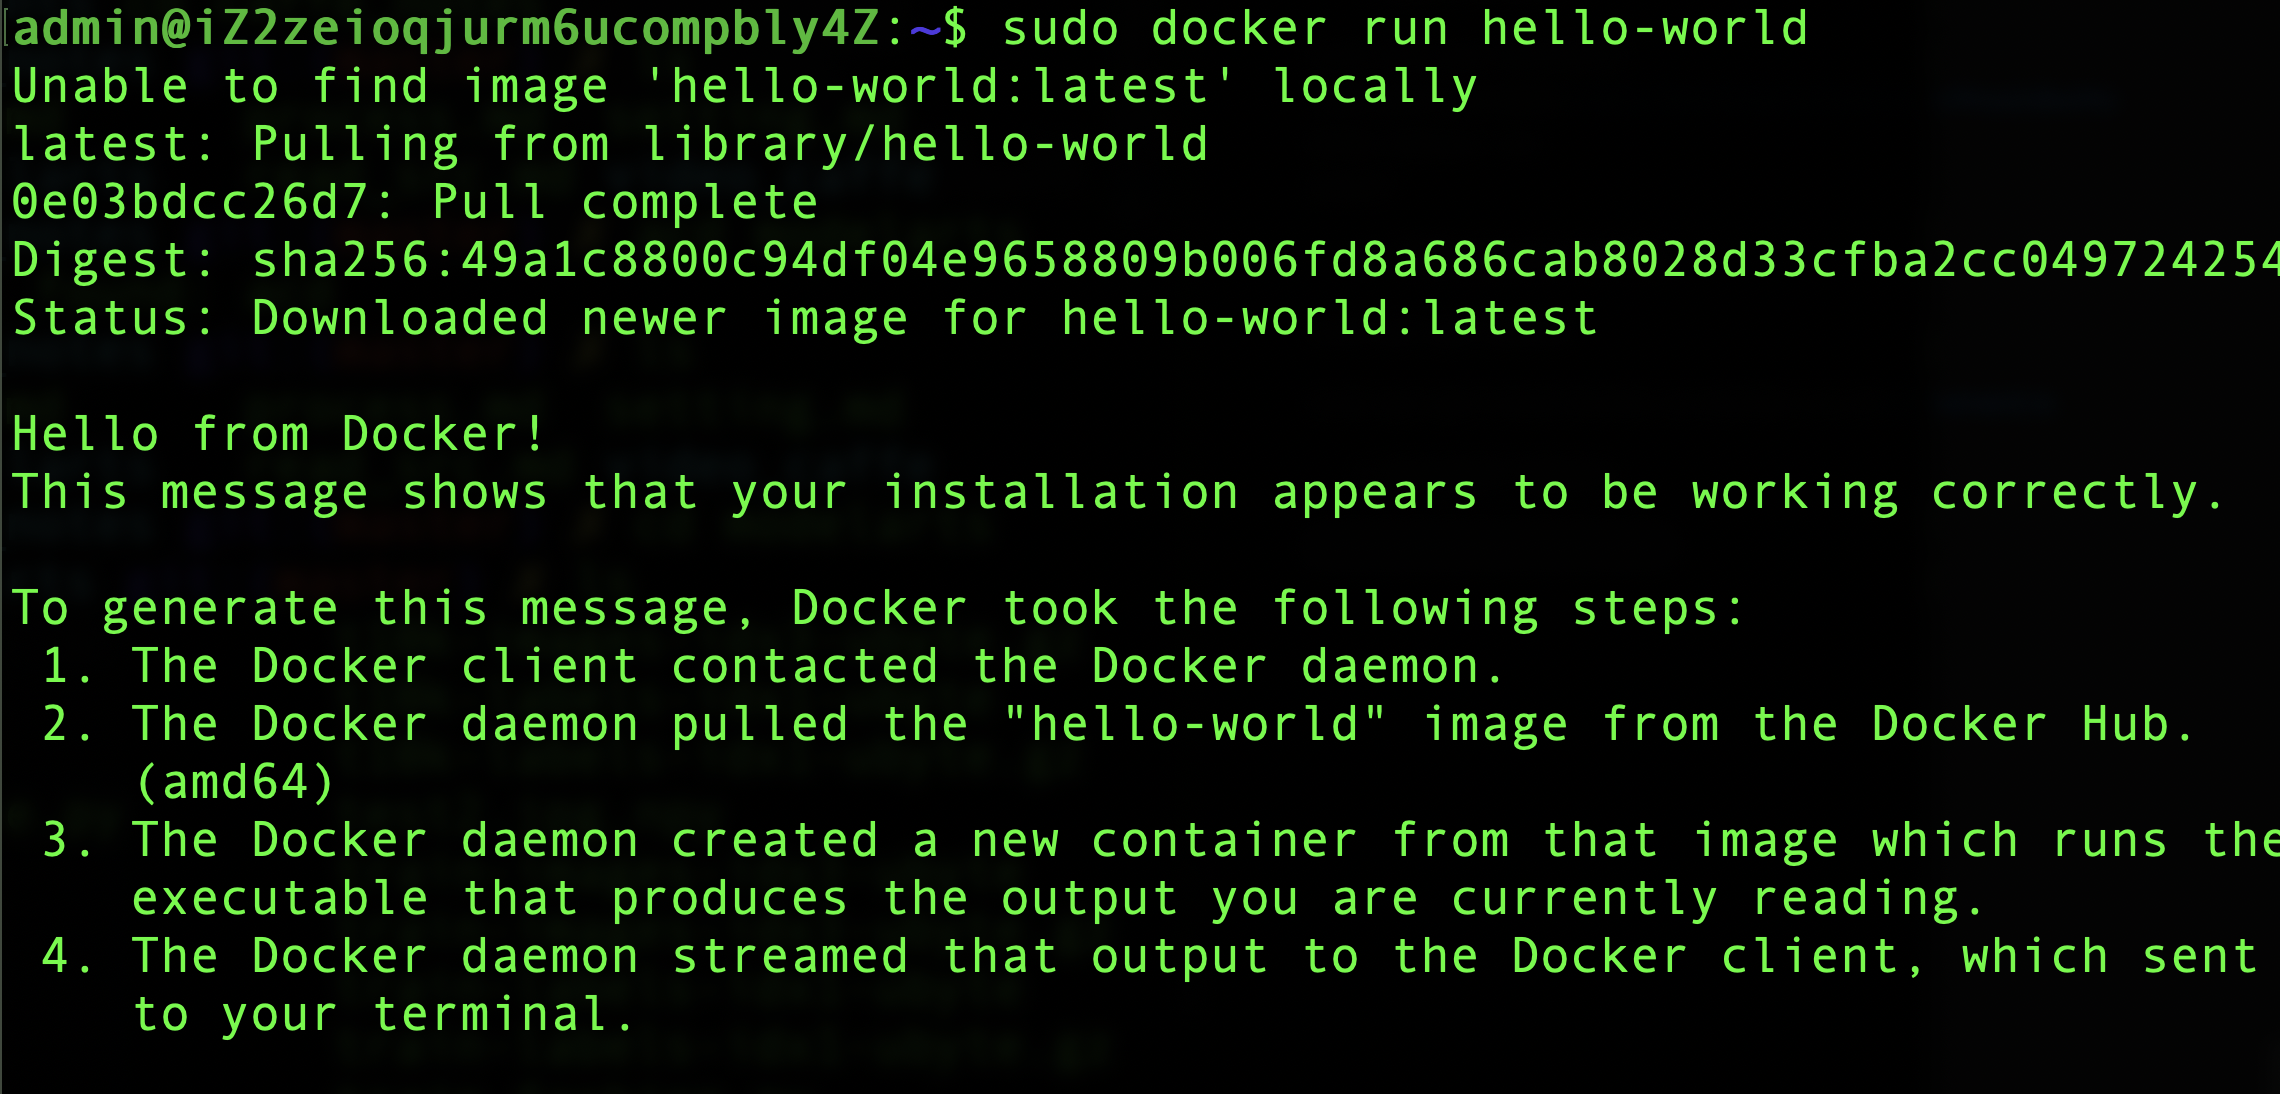
\includegraphics[scale=0.3]{./assets/docker_hw.png}  

\subsection{制作并上传自定义镜像}

1. 编写自定义镜像的 Dockerfile

训练作业的自定义镜像需要以基础镜像为基础。根据

docker pull \url{swr.<region>.myhuaweicloud.com/<image org>/custom-<processor type>-[<cuda version>]-base:<image tag>} 格式。

我们先编写Dockerfile文件。

\lstset{language=bash}
\begin{lstlisting}
FROM swr.cn-north-1.myhuaweicloud.com/eiwizard/custom-gpu-cuda9-inner-moxing-cp36:1.2
ENV BUILD_PATH /root/work

RUN pip install -i https://pypi.tuna.tsinghua.edu.cn/simple pip -U && \
    pip config set global.index-url https://pypi.tuna.tsinghua.edu.cn/simple && \
    pip install --upgrade pip && pip --no-cache-dir install numpy==1.15 tensorflow-gpu==1.15 && \
        echo success
\end{lstlisting}

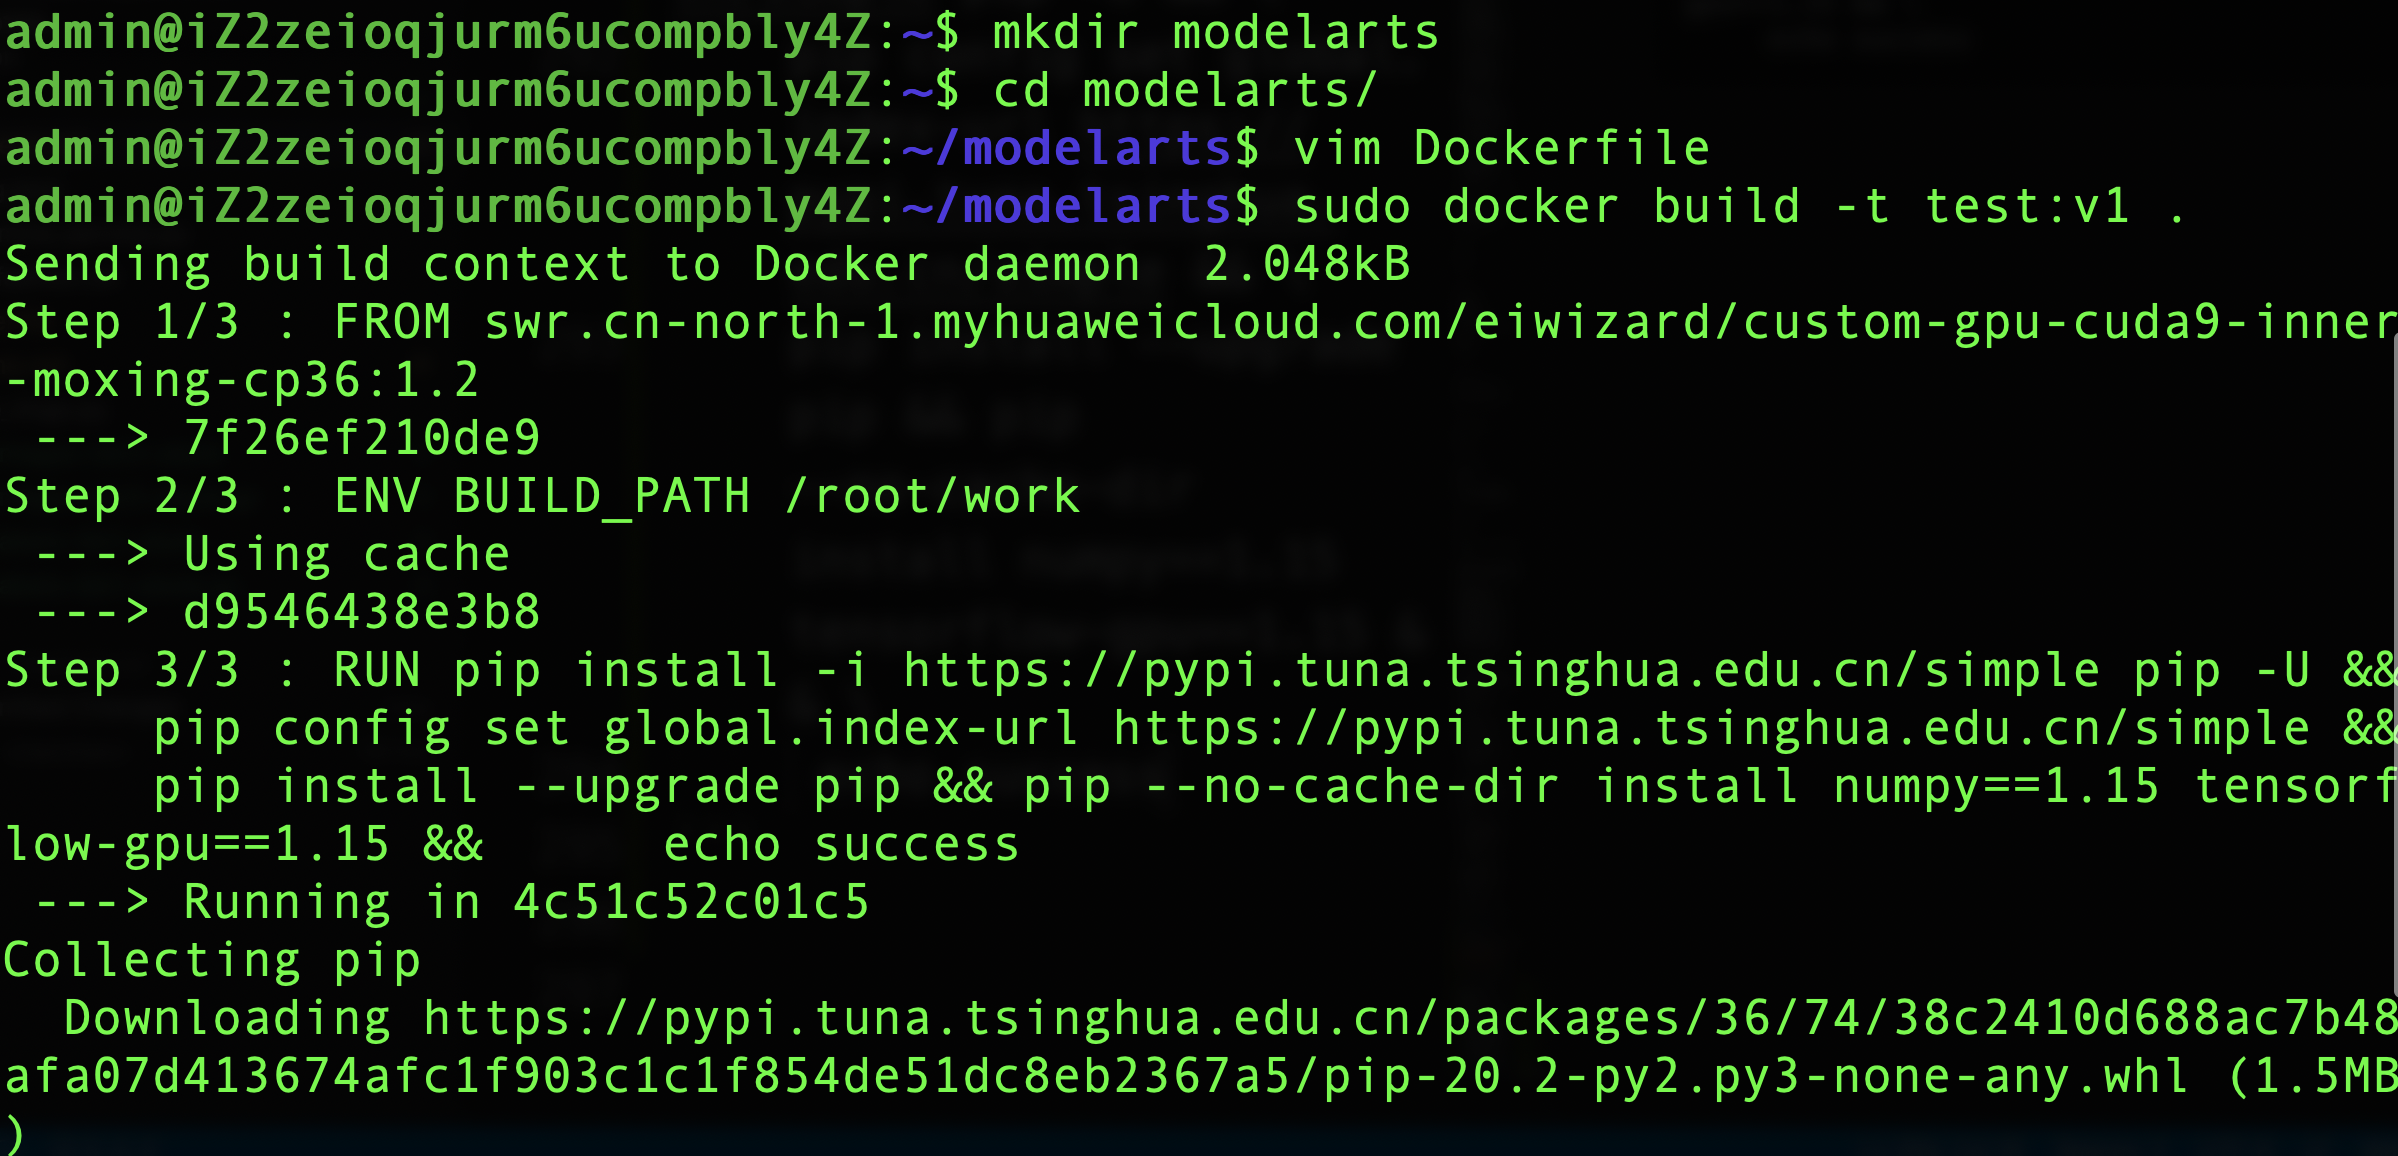
\includegraphics[scale=0.3]{./assets/docker_03.png}  

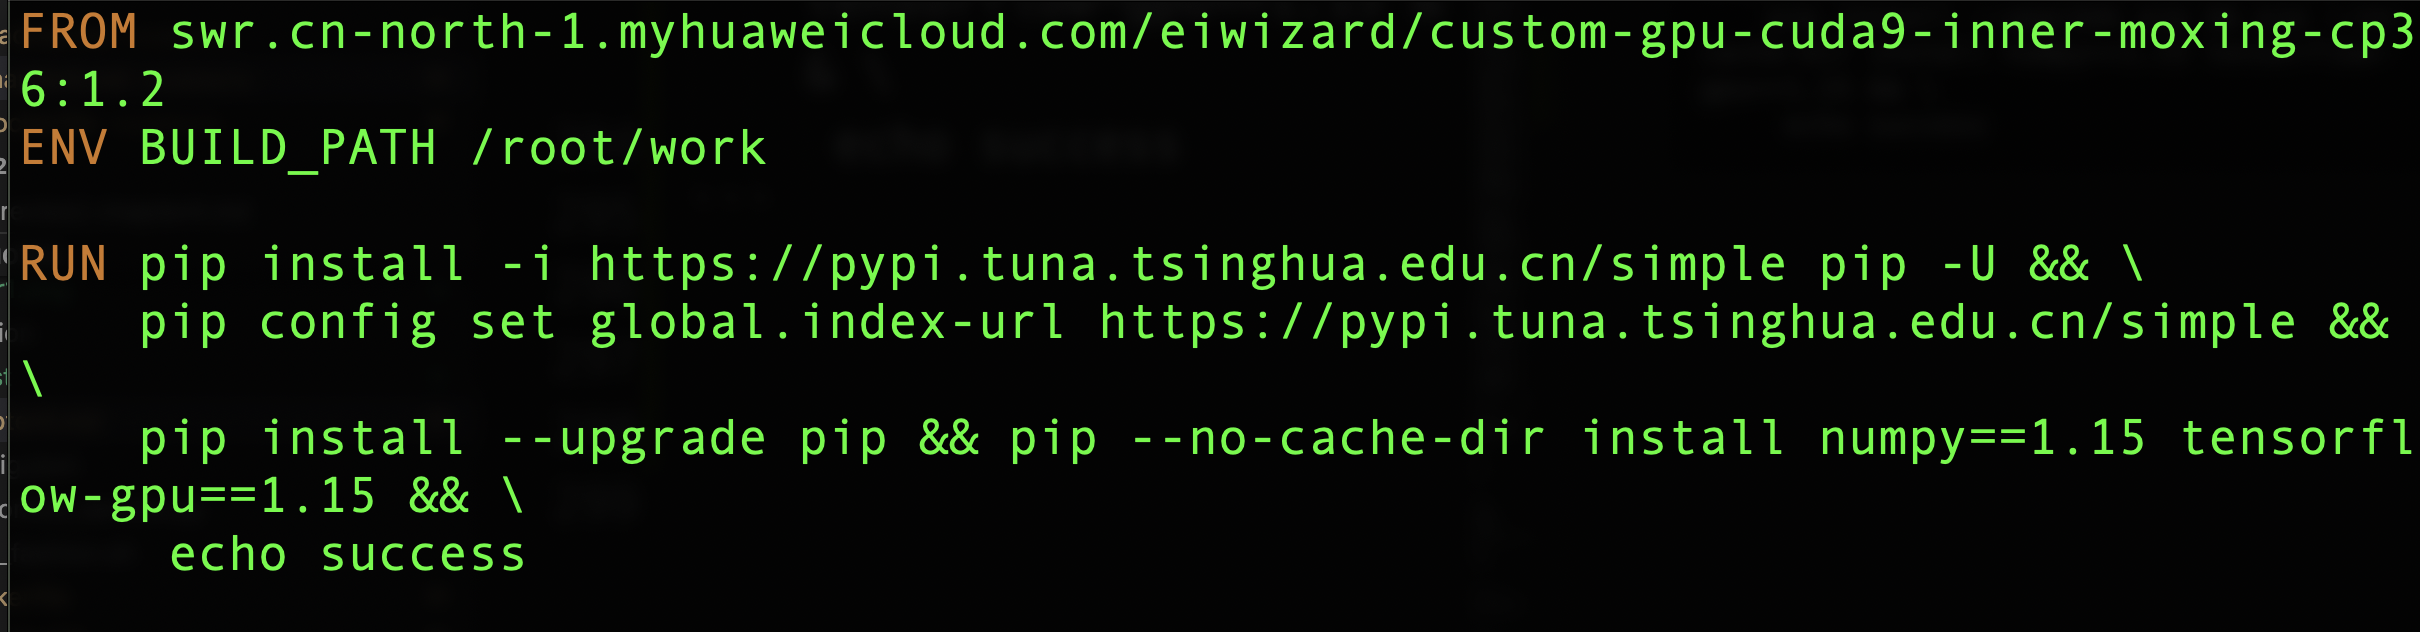
\includegraphics[scale=0.3]{./assets/docker_04.png}  

\subsection{推送镜像至SWR}

在SWR界面上创建一个组织,然后获取SWR登录指令.

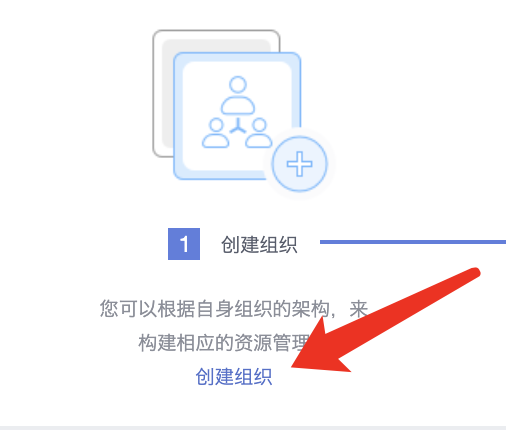
\includegraphics[scale=0.6]{./assets/docker_05.png}  

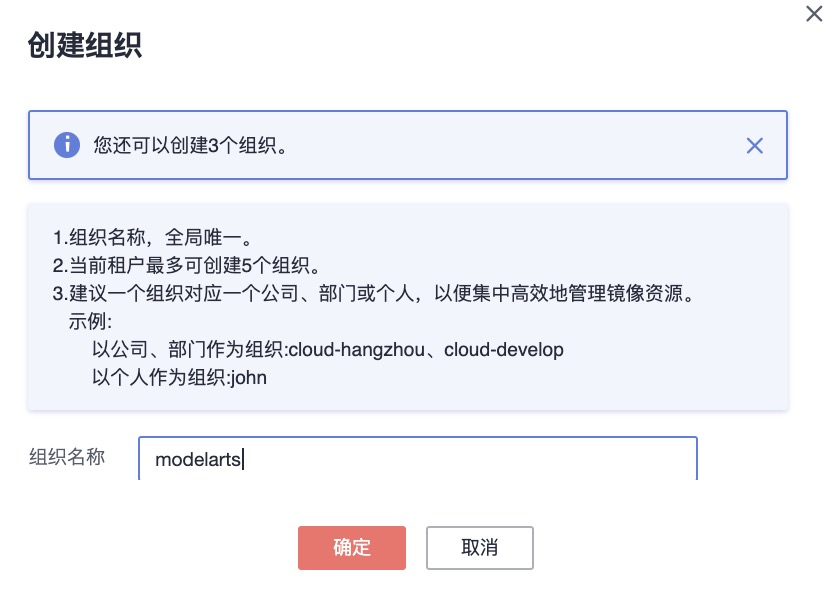
\includegraphics[scale=0.4]{./assets/docker_06.png}  

点击右上角登录指令,单击复制docker login指令。docker login指令末尾的域名即为当前镜像仓库地址,记录该地址。

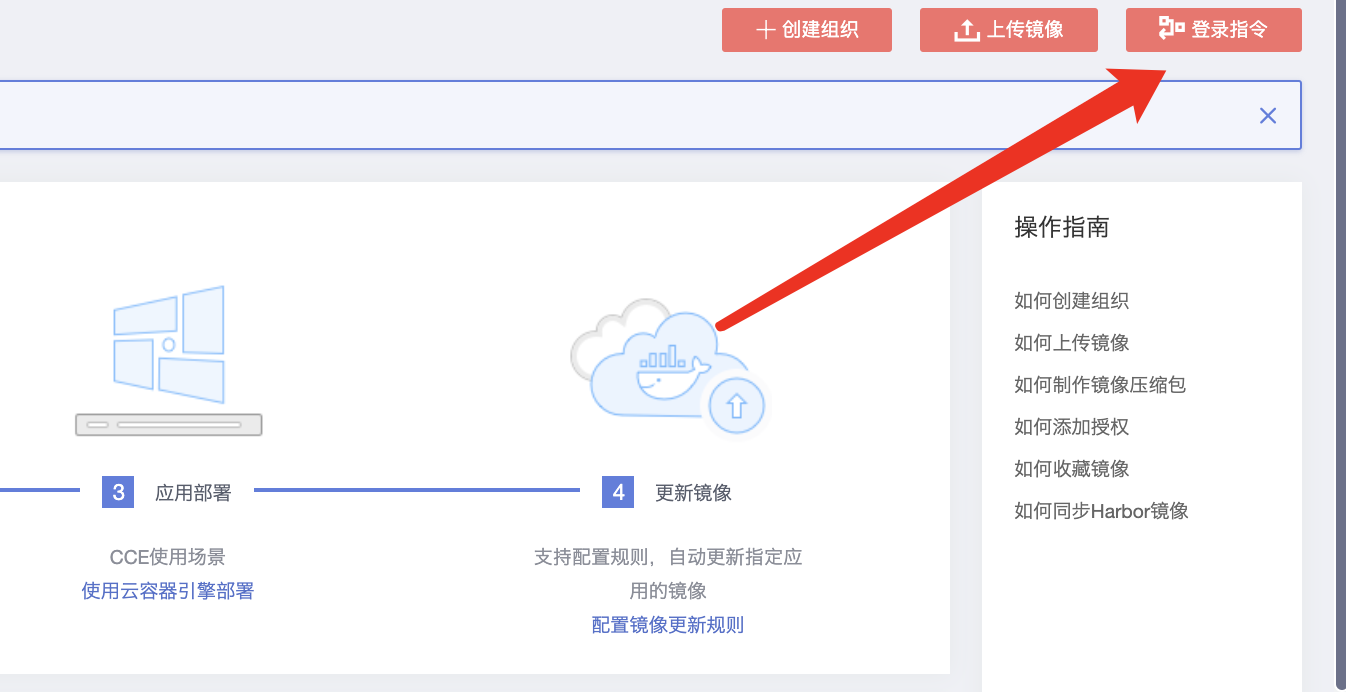
\includegraphics[scale=0.6]{./assets/docker_07.png}  

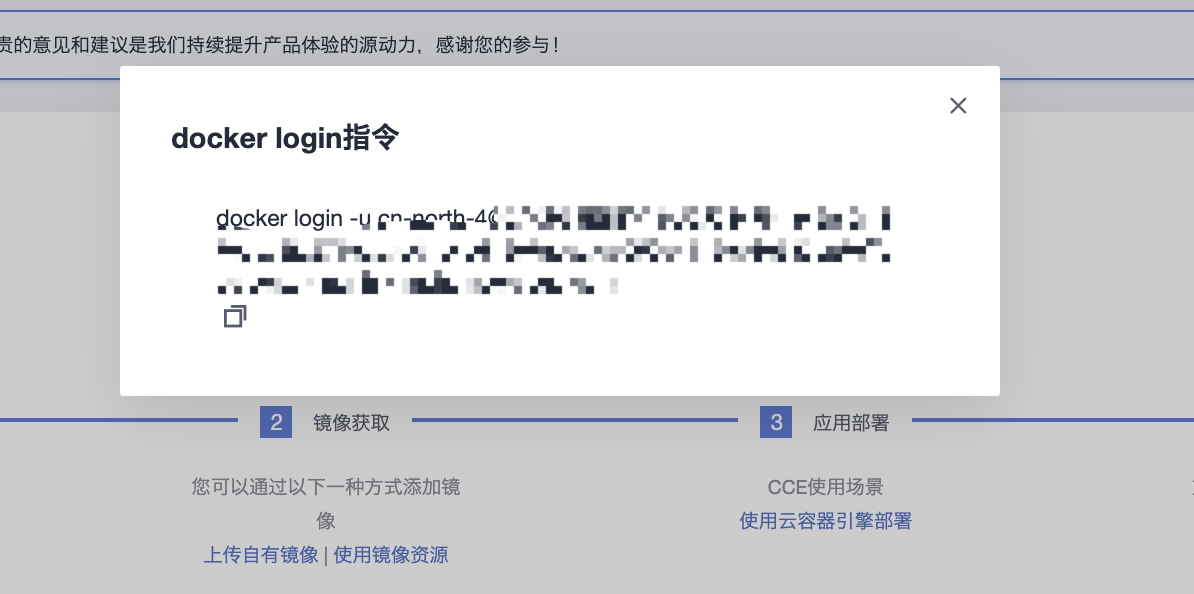
\includegraphics[scale=0.6]{./assets/docker_08.png}  

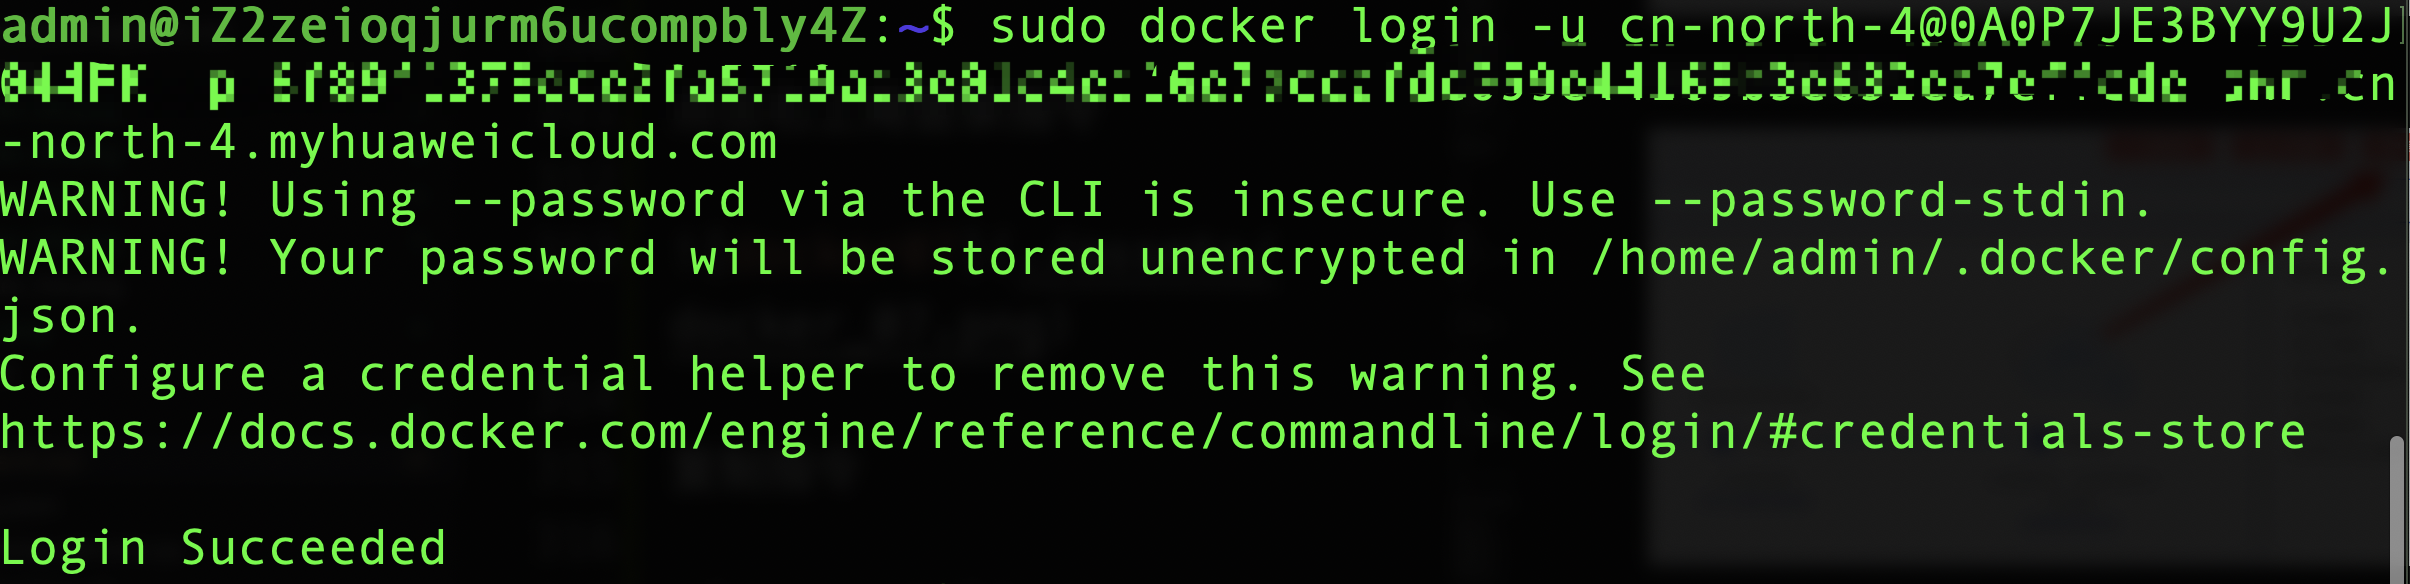
\includegraphics[scale=0.3]{./assets/docker_09.png}  

在安装docker的机器给test:v1镜像打标签。

docker tag [镜像名称:版本名称] [镜像仓库地址]/[组织名称]/[镜像名称:版本名称]

样例如下:

sudo docker tag test:v1 \url{swr.cn-north-4.myhuaweicloud.com/modelarts/test:v1}

其中:

\url{swr.cn-north-4.myhuaweicloud.com}为容器镜像服务的镜像仓库地址。

modelarts为组织名称,如果该组织还没有创建,容器镜像服务会根据组织名称自动创建一个组织。

test:v1为镜像名称和版本号。

上传镜像至镜像仓库。

docker push [镜像仓库地址]/[组织名称]/[镜像名称:版本名称]

样例如下:

sudo docker push \url{swr.cn-north-4.myhuaweicloud.com/modelarts/test:v1}

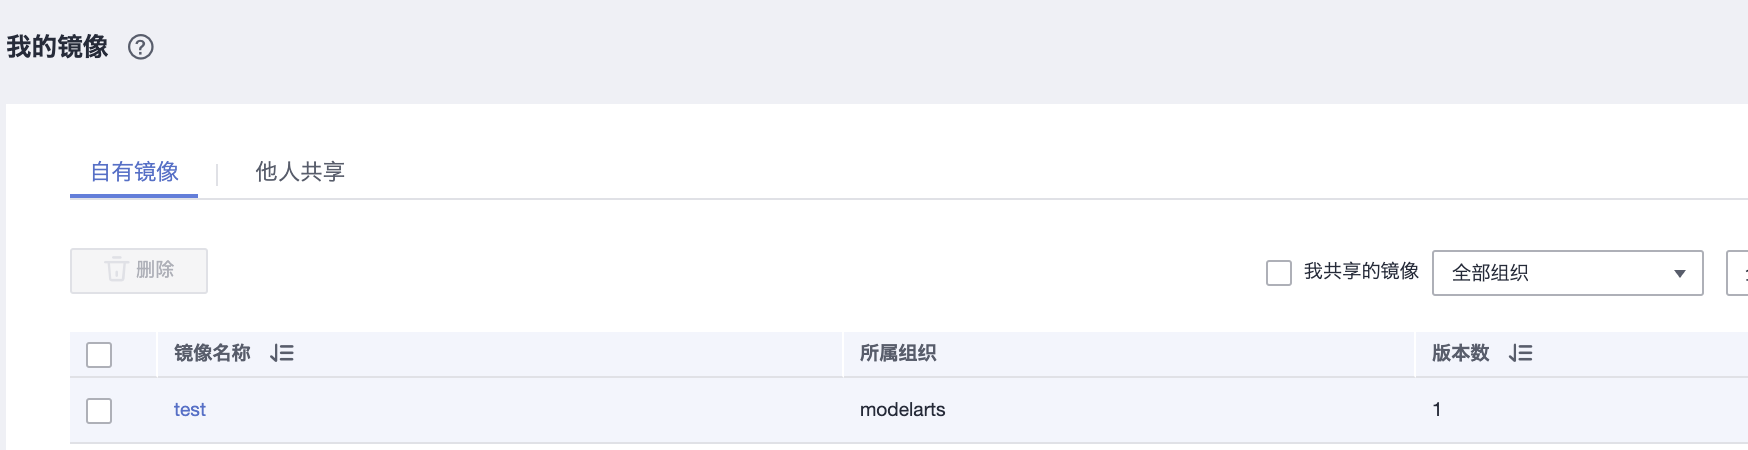
\includegraphics[scale=0.5]{./assets/docker_11.png}  

这样就上传成功了。

\subsection{在ModelArts中使用自定义镜像创建作业}

\subsubsection{创建自定义镜像训练用户作业}

将"mnist\_softmax.py"和训练数据上传至OBS。将脚本和数据都放在代码目录下,以便直接下载到容器中。

启动脚本存储路径为:\url{obs://obs-fashion/new/mnist/mnist_softmax.py}

训练数据存储路径为:\url{obs://modelarts2test/mnist/data}

\lstset{language=python}
\begin{lstlisting}
# mnist_softmax.py
from __future__ import absolute_import
from __future__ import division
from __future__ import print_function

import argparse
import sys

import os
from tensorflow.examples.tutorials.mnist import input_data

import tensorflow as tf

FLAGS = None


def main(_):
    # Import data

    mnist = input_data.read_data_sets(FLAGS.data_dir, one_hot=True)
    # Create the model
    x = tf.placeholder(tf.float32, [None, 784])
    W = tf.Variable(tf.zeros([784, 10]))
    b = tf.Variable(tf.zeros([10]))
    y = tf.matmul(x, W) + b

    # Define loss and optimizer
    y_ = tf.placeholder(tf.float32, [None, 10])

    cross_entropy = tf.reduce_mean(
        tf.nn.softmax_cross_entropy_with_logits(labels=y_, logits=y))
    train_step = tf.compat.v1.train.GradientDescentOptimizer(0.5).minimize(cross_entropy)

    sess = tf.compat.v1.InteractiveSession()
    tf.compat.v1.global_variables_initializer().run()
    # Train
    print('Training ................')
    for _ in range(1000):
        batch_xs, batch_ys = mnist.train.next_batch(100)
        sess.run(train_step, feed_dict={x: batch_xs, y_: batch_ys})

    # Test trained model
    correct_prediction = tf.equal(tf.argmax(y, 1), tf.argmax(y_, 1))
    accuracy = tf.reduce_mean(tf.cast(correct_prediction, tf.float32))
    print(sess.run(accuracy, feed_dict={x: mnist.test.images,
                                        y_: mnist.test.labels}))

if __name__ == '__main__':
    parser = argparse.ArgumentParser()
    parser.add_argument('--data_dir', '--data_url', type=str, default='/home/work/user-job-dir/fashion_data',
                        help='Directory for storing input data')
    FLAGS, unparsed = parser.parse_known_args()
    tf.app.run(main=main, argv=[sys.argv[0]] + unparsed)
\end{lstlisting}

创建自定义镜像训练作业,"镜像地址"、"代码目录"和"运行命令"参考如下信息填写,“数据存储位置”和“训练输出位置”请根据实际情况填写。

"镜像地址":填写刚上传镜像的"SWR\_URL"。

"代码目录":选择存储在OBS的训练代码。例如\url{obs://obs-fashion/new/mnist/}为代码根目录,\url{obs://obs-fashion/new/mnist/mnist_softmax.py}为代码启动文件。

在训练作业实际启动之前,ModelArts自动将“代码目录”下的所有内容递归下载到本地路径,存放代码的本地路径为 “\${ModelArts 训练固定的工作目录}/\${代码根目录的最后一级名称}”。当前“\${ModelArts 训练固定的工作目录}” 为 “\url{/home/work/user-job-dir}”。例如,“代码目录”选择“\url{obs://obs-fashion/new/mnist/}”时,本地代码目录对应为“\url{/home/work/user-job-dir/mnist/}”,代码启动文件位于 \url{/home/work/user-job-dir/mnist/mnist_softmax.py}。

其中,“\url{/home/work/user-job-dir/mnist/mnist_softmax.py}”为下载下来训练脚本的位置,“--data\_url \url{/home/work/user-job-dir/mnist/data}”为数据的位置。由于已经把数据放在代码目录中,容器已经下载了代码目录,所以直接使用本地的。

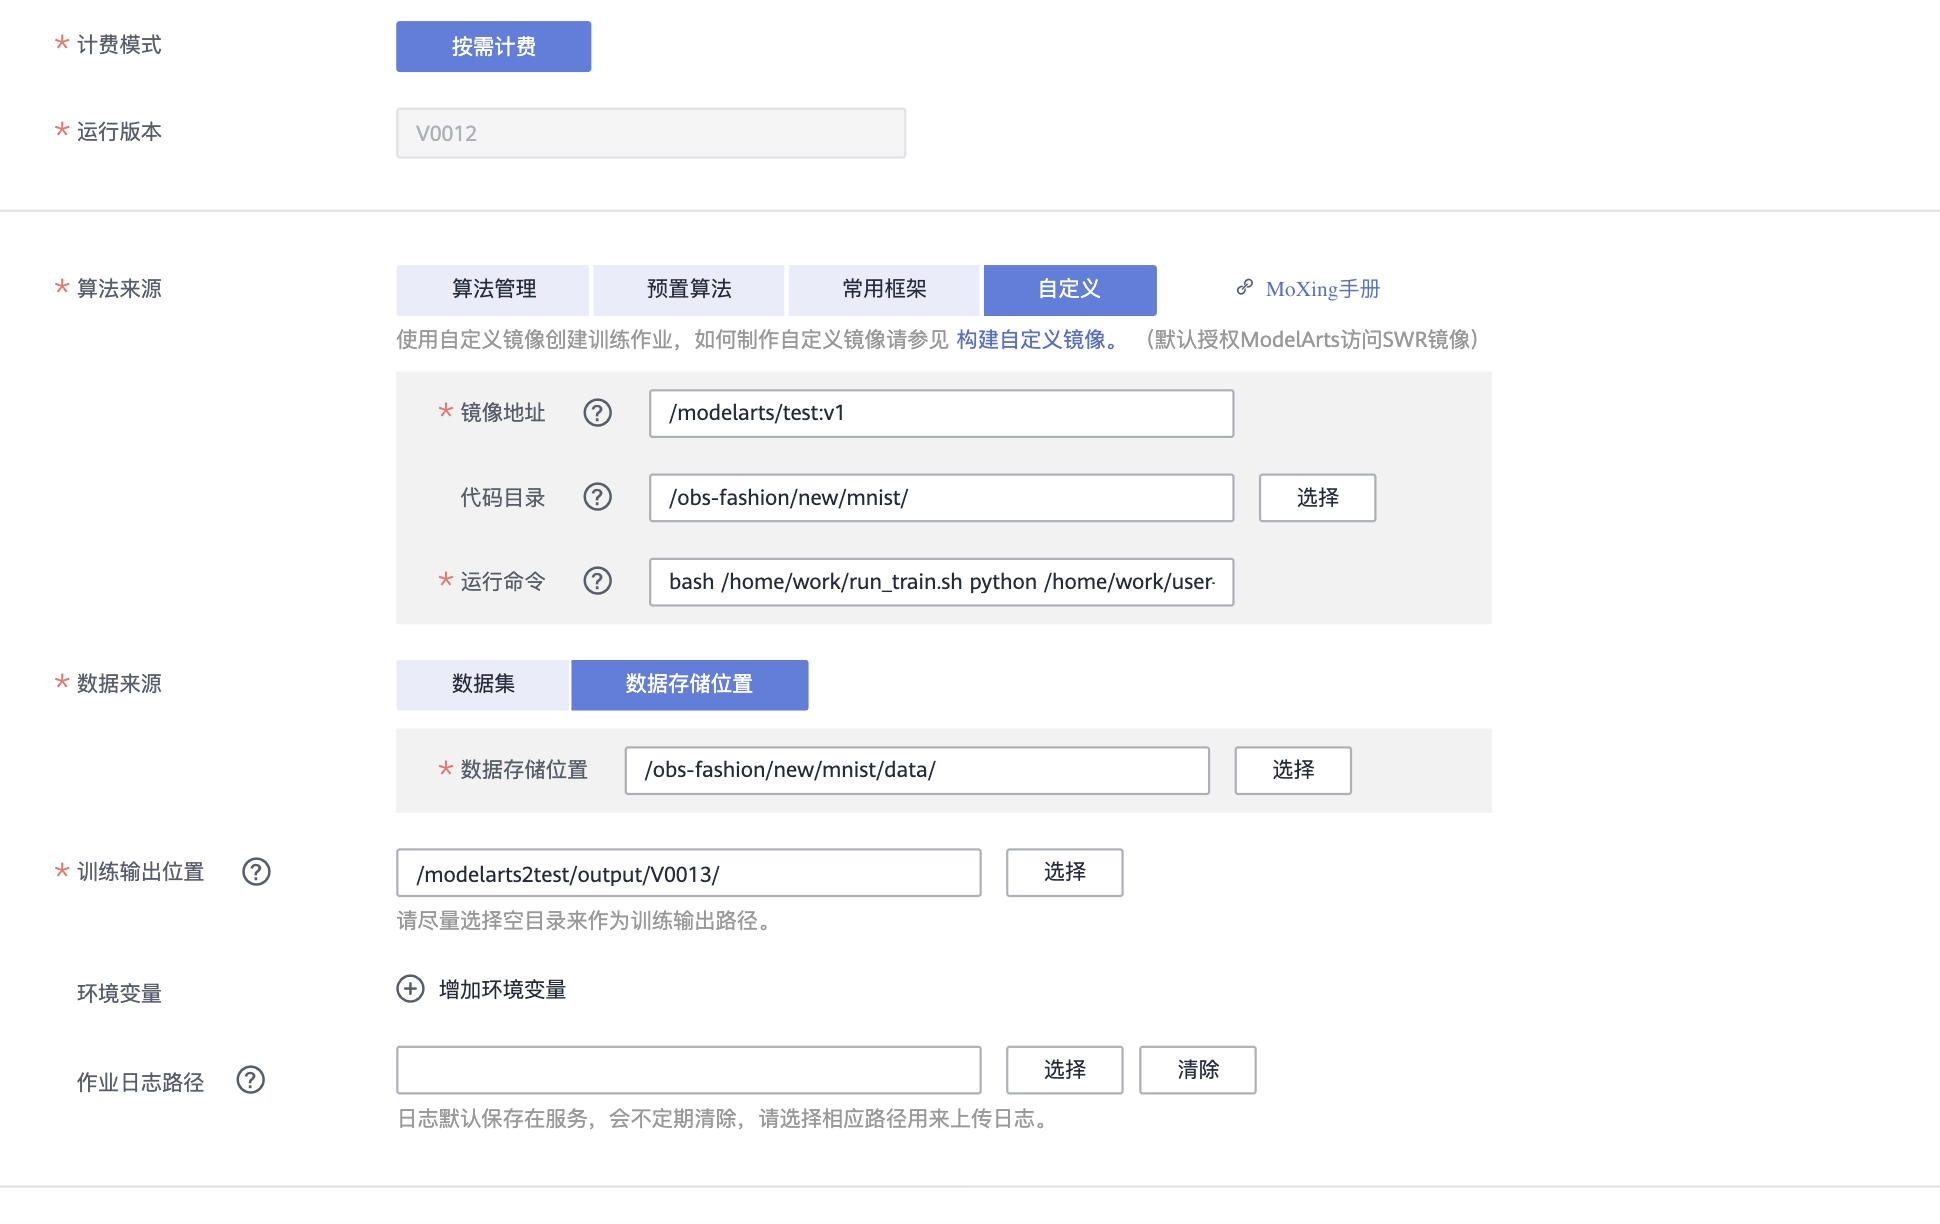
\includegraphics[scale=0.5]{./assets/kernel_02.png}  


\section{强化学习实验}

\subsection{1. 安装gym环境}

openai gym工具箱提供了一系列物理仿真环境,游戏,机器人仿真。我们可以基于gym提供的环境来设计强化学习的agent。

\lstset{language=python}
\begin{lstlisting}
!pip install --upgrade pip
!pip install 'gym[atari]'
\end{lstlisting}

引入包所需的包

\lstset{language=python}
    \begin{lstlisting}
    import numpy as np
    import pandas as pd
    import tensorflow as tf
import matplotlib.pyplot as plt
from sklearn.utils import shuffle
import gym
\end{lstlisting}

一些超参数设置

\lstset{language=python}
\begin{lstlisting}
end_game_reward = -100
hidden_layers = [12,12]
gamma = 0.99
learning_rate = 0.0001
internal = 100
env_name = 'SpaceInvaders-v0'
env = gym.make(env_name)
w,h,d = env.observation_space.shape
state_num = w * h * d
\end{lstlisting}


我们分别打印出可用 action,可用的 observation, observation 最高值,observation 最低值

\lstset{language=python}
\begin{lstlisting}
print(env.action_space)
print(env.observation_space)
print(env.observation_space.high) 
print(env.observation_space.low)
\end{lstlisting}

我们来定义gradient policy的类

\lstset{language=python}
\begin{lstlisting}
class PolicyGradient:
    def __init__(self, state_size, num_of_actions, hidden_layers, learning_rate):
        self.states = tf.placeholder(shape=(None, state_size), dtype=tf.float32, name='input_observation') ## `接收 observation`
        self.acc_r = tf.placeholder(shape=None, dtype=tf.float32, name='accumalated_rewards') # `接收每个 state-action 所对应的 value (通过 reward 计算)`
        self.actions = tf.placeholder(shape=None, dtype=tf.int32, name='actions') ## `接收action`
        layer = self.states
        ## `堆叠神经网络层`
        for i in range(len(hidden_layers)):
            layer = tf.layers.dense(inputs=layer, units=hidden_layers[i], activation=tf.nn.relu,
                                    kernel_initializer=tf.contrib.layers.xavier_initializer(),
                                    name='hidden_layer_{}'.format(i+1))
        self.last_layer = tf.layers.dense(inputs=layer, units=num_of_actions, activation=tf.nn.tanh,
                                          kernel_initializer=tf.contrib.layers.xavier_initializer(),
                                          name='output')
        self.action_prob = tf.nn.softmax(self.last_layer)  # `激励函数 softmax 出概率`
        self.log_policy = tf.nn.sparse_softmax_cross_entropy_with_logits(logits=self.last_layer, labels=self.actions) # `所选 action 的概率 -log 值`
        # log_policy = tf.reduce_sum(-tf.log(self.log_policy)*tf.one_hot(self.actions, self.num_of_actions), axis=1)
        self.cost = tf.reduce_mean(self.acc_r * self.log_policy) 
        # (acc_r = `本`reward + `衰减的未来`reward) `引导参数的梯度下降`
         # `最大化 总体` reward (acc_r * log_policy) `就是在最小化` -(acc_r * log_policy), `而 tf 的功能里只有最小化 loss`
        self.optimizer = tf.train.AdamOptimizer(learning_rate=learning_rate).minimize(self.cost)
\end{lstlisting}

接下来我们定义policygradient:
\lstset{language=python}
\begin{lstlisting}
    pg = PolicyGradient(state_size=state_num, num_of_actions=env.action_space.n,
    hidden_layers=hidden_layers, learning_rate=learning_rate)
\end{lstlisting}

然后进入主循环

\lstset{language=python}
\begin{lstlisting}
    from scipy.stats import zscore
    def print_stuff(s, every=100):
        if game % every == 0 or game == 1:
            print(s)
    sess = tf.Session()
    sess.run(tf.global_variables_initializer())
    data = pd.DataFrame(columns=['game','steps','cost'])
    
    for g in range(1500):
        game = g+1
        done = False
        ## init env
        observation = env.reset()
        states = [] 
        rewards = [] 
        actions = []
        steps = 0
        print_stuff('Starting game {}'.format(game))
        while not done:
            steps += 1
            observation = observation.flatten()[np.newaxis, :]
            
            probs = sess.run(pg.action_prob, feed_dict={pg.states: observation}).flatten()
            # `选择action`
            action = np.random.choice(env.action_space.n, p=probs)
    
            ## `根据这个action, 给出下一个state,reward,是否游戏结束`
            next_state, r, done, _ = env.step(action)
            if done and steps < env._max_episode_steps: r = end_game_reward
            
            # `存储这一回合的数据`
            states.append(observation)
            rewards.append(r)
            actions.append(action)
            observation = next_state
        print_stuff('Game {g} has ended after {s} steps.'.format(g=game, s=steps))
        
        discounted_acc_rewards = np.zeros_like(rewards)
        s = 0.0
        for i in reversed(range(len(rewards))):
            s = s * gamma + rewards[i]
            discounted_acc_rewards[i] = s
        discounted_acc_rewards = zscore(discounted_acc_rewards)
        
        states, discounted_acc_rewards, actions = shuffle(states, discounted_acc_rewards, actions)
        # `用一轮数据更新policy gradient 网络`
        c, _ = sess.run([pg.cost, pg.optimizer], feed_dict={pg.states: np.squeeze(states), 
                                                            pg.acc_r: discounted_acc_rewards,
                                                            pg.actions: actions})    
        
        print_stuff('Cost: {}\n----------'.format(c))
        data = data.append({'game':game, 'steps':steps, 'cost':c}, ignore_index=True)
\end{lstlisting}

用视频捕捉一下,然后显示

\lstset{language=python}
\begin{lstlisting}
from gym import wrappers
env = wrappers.Monitor(env, "./gym-results", force=True)
env.reset()
for _ in range(5000):
    action = env.action_space.sample()
    observation, reward, done, info = env.step(action)
    if done: break
env.close()
\end{lstlisting}

\lstset{language=python}
\begin{lstlisting}
import io
import base64
from IPython.display import HTML

video = io.open('./gym-results/openaigym.video.%s.video000000.mp4' % env.file_infix, 'r+b').read()
encoded = base64.b64encode(video)
HTML(data='''
    <video width="360" height="auto" alt="test" controls><source src="data:video/mp4;base64,{0}" type="video/mp4" /></video>'''
.format(encoded.decode('ascii')))
\end{lstlisting}

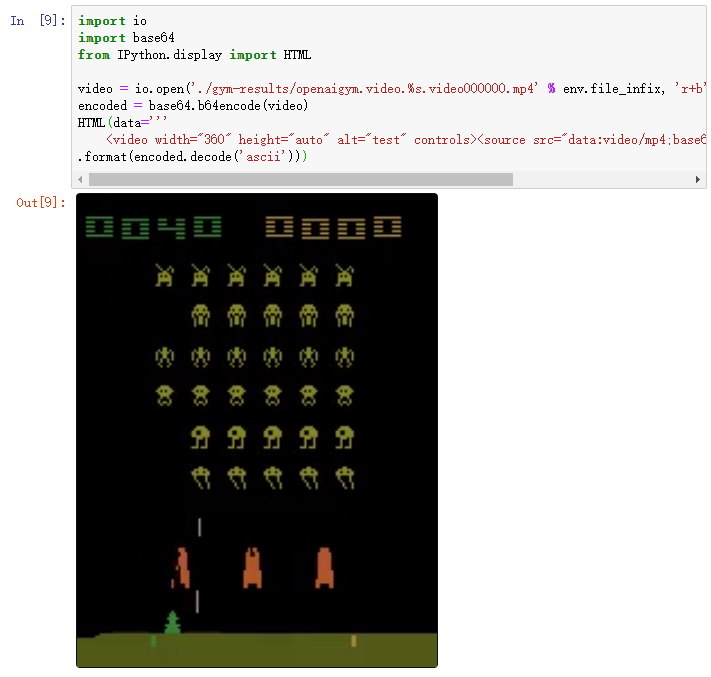
\includegraphics[scale=0.5]{./assets/rl_game.png}  

\subsection{标题}

\chapter{标题}
\section{标题}

\subsection{标题}


\chapter*{参考文献}

\end{document}